\documentclass[10pt]{article}
\usepackage[utf8]{inputenc}
\usepackage{amscd}
\usepackage{amsmath}
\usepackage{amssymb}
\usepackage{amsthm}
\usepackage{listings}
\usepackage{enumerate}
\usepackage{graphicx}

\graphicspath{{images/}}

\textwidth=15cm \textheight=22cm \topmargin=0.5cm \oddsidemargin=0.5cm \evensidemargin=0.5cm

\newcommand{\sk}{\vskip 10mm}
\newcommand{\bb}[1]{\mathbb{#1}}
\newcommand{\ra}{\rightarrow}

\theoremstyle{plain}
\newtheorem{problem}{Problem}
\newtheorem{lemma}{Lemma}[problem]

\theoremstyle{remark}
\newtheorem{tpart}{}[problem]
\newtheorem*{ppart}{}

\begin{document}

\begin{problem}
  Verify explicitly that $\partial^2=0$.
\end{problem}

\begin{proof}
  Consider $[v_1,\ldots,v_n]$. Then
  \[ \partial^2([v_1,\ldots,v_n])=
    \sum_{j<i}(-1)^{i+j}[v_1,\ldots,\hat{v_j},\ldots,\hat{v_i},\ldots, v_n]
    + \sum_{i<j}(-1)^{i+j-1}[v_1,\ldots,\hat{v_i},\ldots,\hat{v_j},\ldots,v_n]\]
  Then if we swap $i,j$ for the first sum and pull out a negative we get
  \begin{align*}
    \partial^2([v_1,\ldots,v_n]) &=\sum_{j<i}(-1)^{i+j}[v_1,\ldots,\hat{v_j},\ldots,\hat{v_i},\ldots, v_n]
                          + \sum_{i<j}(-1)^{i+j-1}[v_1,\ldots,\hat{v_i},\ldots,\hat{v_j},\ldots,v_n]\\
                        & = -\sum_{i<j}(-1)^{j+i-1}[v_1,\ldots,\hat{v_i},\ldots,\hat{v_j},\ldots, v_n]
                          + \sum_{i<j}(-1)^{i+j-1}[v_1,\ldots,\hat{v_i},\ldots,\hat{v_j},\ldots,v_n]\\
                        &= 0
  \end{align*}

  Therefore $\partial^2= 0$.
\end{proof}

\sk

\begin{problem}
  Compute the simplicial homology of the Klein bottle using the
  $\Delta$-complex structure, with two simplices of dimension 2.
\end{problem}

\begin{proof}
  \verb|A:|
  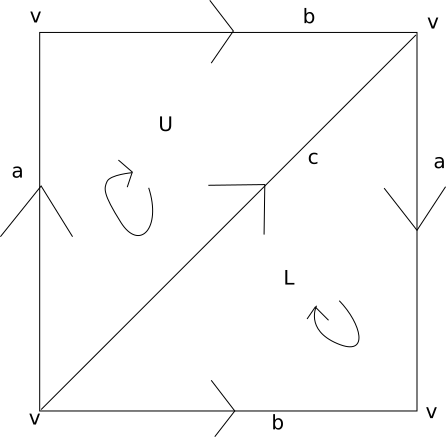
\includegraphics[scale=.5]{klein}

  First we'll list the images of all the various simplices.
  \begin{align*}
    \partial U &= a+b-c\\
    \partial L &= a-b+c\\
    \partial a &= v-v&=0\\
    \partial b &= v-v&=0\\
    \partial c &= v-v&=0\\
    \partial v &= 0\\
  \end{align*}
  For $H_2(K)=\frac{\ker \partial}{\text{Im} \partial}$ the image is trivial as there as
  there are no 3 simplices and the kernel is when $\partial(pU+qL)=(p+q)a+(p-q)b+(q-p)c$
  is zero which only occurs if $p=q=0$. Therefore $H_2(K)=0$.

  For $H_1(K)$ the kernel is the free abelian group on $a,b,c$ and the image
  is generated by $(a+b-c)$ and $a-b+c$. So our group is the abelian group
  generated by $\langle a,b,c|a+b=c,a+c=b\rangle$. We can simplify to remove $c$ and
  get $\langle a,b|2a\rangle$. Therefore $H_1(K)=\bb{Z}\oplus\bb{Z}_2$.

  For $H_0(K)$ the image is trivial and the kernel is the whole space. Thus
  $H_0(K)=\bb{Z}$.
\end{proof}

\sk

\begin{problem}
  Show that if $G$ is a finitely generated free abelian group
  and $H\subset G$ is a subgroup, then there is a basis $g_1,\ldots,g_n$
  for $G$ and integers $p_1,\ldots,p_k$ with $k\leq n$ such that
  each $p_i$ divides $p_{i+1}$, and such that $p_1g_1,\ldots,p_kg_k$ is
  a basis for $H$. We say that these bases for $G$ and $H$ are
  stacked. Conclude that
  \[ G/H\cong \bb{Z}_{p_1}\oplus\cdots\oplus\bb{Z}_{p_k}\oplus\bb{Z}^{n-k} \]
  In particular, every finitely generated abelian group is a
  direct sub of cyclic groups. (Hint: You may find it helpful to
  use the fact that subgroups of free abelian groups are themselves
  free abelian.)
\end{problem}

\begin{proof}
  By the structure theorem for finitely generated modules over a PID and the
  fact that abelian groups are $\bb{Z}$-modules there exists a basis of
  $G=\langle g_1,\ldots,g_n\rangle$ such that $H=\langle p_1g_1,\ldots,p_kg_k\rangle$ where
  $p_i|p_{i+1}$. If we then look at the quotient $G/H$ we get
  \[ G/H\cong \langle g_1,\ldots,g_n|p_ig_i=0:1\leq i\leq k\rangle \]
  However this implies that the subgroup generated by $g_i$ will be
  $\bb{Z}_{p_i}$ for $i\leq k$ and $\bb{Z}$ otherwise. Since the group is abelian
  we can then conclude that
  \[ G/H\cong \bb{Z}_{p_1}\oplus\cdots\oplus\bb{Z}_{p_k}\oplus\bb{Z}^{n-k} \]
\end{proof}

\sk

\begin{problem}
  If $i:A\rightarrow X$ is the inclusion of a retract of $X$, show that
  $i_*:H_k(A)\rightarrow H_k(X)$ is a monomorphism onto a direct summand of
  $H_k(X)$. If $A$ is deformation retract of $X$, show that
  $i_*$ is an isomorphism.
\end{problem}

\begin{proof}
  Let $i:A\rightarrow X$ be the inclusion and $r:X\rightarrow A$ the retract of $X$ onto $A$.
  By definition $r\circ i =id_A$ which implies that the map induced on the
  homology $r_*\circ i_* = id_*$. Since $i_*$ has a left inverse it must be
  injective. Therefore the map induced by the inclusion of a retract is
  injective.

  Now suppose that $A$ is a deformation retract of $X$. Then $r$ is
  homotopic to $id_X$. Then we have that $i\circ r$ is homotopic to $id_X$
  which means that $i$ is a homotopy equivalence and as such induces
  an isomorphism on the homology (Hatcher 2.11) of $A$ and $X$.
\end{proof}

\sk

\begin{problem}
  Show that it is impossible to retract the $n-$ball $B^n$ onto its
  $n-1$-sphere boundary $\partial B^n=S^{n-1}$.
\end{problem}

\begin{proof}
  Since $B^n$ is contractible $H_k(B^n)=0$ for all $k$. If there existed
  a retract of $B^n$ onto $S^1$ this would imply that
  there exists an injective function from $H_{n-1}(S^{n-1})=\bb{Z}$
  to the trivial group which is a contradiction.

  Therefore there is no deformation retract from $B^n$ to $S^{n-1}$.
\end{proof}

\sk

\begin{problem}
  Compute the simplicial homology of the Klein bottle using the
  $\Delta$-complex structure, with two simplices of dimension 2, discussed in
  class.
\end{problem}

\begin{proof}
  \verb|goto A;|
\end{proof}

%%%%%%%%%%%%%%%%%%%%%%%%%%%%%%%%%%%%%%%%%%%%%%%%%%%%%%%%%%%%%%%%%%%%%%%%%%%%%
\end{document}
